\let\negmedspace\undefined
\let\negthickspace\undefined
\documentclass[journal]{IEEEtran}
\usepackage[a5paper, margin=10mm, onecolumn]{geometry}
%\usepackage{lmodern} % Ensure lmodern is loaded for pdflatex
\usepackage{tfrupee} % Include tfrupee package

\setlength{\headheight}{1cm} % Set the height of the header box
\setlength{\headsep}{0mm}     % Set the distance between the header box and the top of the text

\usepackage{gvv-book}
\usepackage{gvv}
\usepackage{cite}
\usepackage{amsmath,amssymb,amsfonts,amsthm}
\usepackage{algorithmic}
\usepackage{graphicx}
\usepackage{textcomp}
\usepackage{xcolor}
\usepackage{txfonts}
\usepackage{listings}
\usepackage{enumitem}
\usepackage{mathtools}
\usepackage{gensymb}
\usepackage{comment}
\usepackage[breaklinks=true]{hyperref}
\usepackage{tkz-euclide} 
\usepackage{listings}
% \usepackage{gvv}                                        
\def\inputGnumericTable{}                                 
\usepackage[latin1]{inputenc}                                
\usepackage{color}                                            
\usepackage{array}                                            
\usepackage{longtable}                                       
\usepackage{calc}                                             
\usepackage{multirow}                                         
\usepackage{hhline}                                           
\usepackage{ifthen}                                           
\usepackage{lscape}
\begin{document}

\bibliographystyle{IEEEtran}
\vspace{3cm}

\title{NCERT-9.5.3}
\author{EE24BTECH11055 - Sai Akhila}
% \maketitle
% \newpage
% \bigskip
{\let\newpage\relax\maketitle}

\renewcommand{\thefigure}{\theenumi}
\renewcommand{\thetable}{\theenumi}
\setlength{\intextsep}{10pt} % Space between text and floats


\numberwithin{equation}{enumi}
\numberwithin{figure}{enumi}
\renewcommand{\thetable}{\theenumi}

% Question
\section*{Question:}
At what points in the interval \sbrak{0, 2\pi}, does the function $\sin(2x)$ attain its maximum value?
%  Solution
\section*{What is the Gradient Descent algorithm?}
Gradient descent is an optimization algorithm used to minimize a function by iteratively moving towards the direction of the steepest descent (the negative gradient) of the function. It is widely used in machine learning and mathematical optimization to minimize loss functions and find optimal parameters.
Below are the steps:\\

\begin{enumerate}
    \item Define the Objective Function:
    \begin{itemize}
        \item Let \brak{f\brak{x}} be the function you want to minimize. Here, \brak{x} can be a scalar or a vector.
    \end{itemize}

    \item Initialize Parameters:
    \begin{itemize}
        \item Start with an initial guess for \brak{x_0}, which is the starting point of the optimization.
    \end{itemize}

    \item Compute the Gradient:
    \begin{itemize}
        \item Calculate the gradient \brak{\nabla f\brak{x_t}} of the function with respect to \brak{x} at the current position \brak{x_t}. The gradient points in the direction of the steepest increase.
    \end{itemize}

    \item Update Parameters:
    \begin{itemize}
        \item Update \brak{x_t} using the gradient descent formula:
        \begin{align}
            x_{t+1} = x_t - \eta \cdot \nabla f\brak{x_t}
        \end{align}
        where:
        \begin{itemize}
            \item \brak{\eta} is the learning rate, which determines the step size.
        \end{itemize}
        In this case, we have the equation as:
        \begin{align}
		x_{t+1}=x_t- \eta \cdot 2\cos{2x_t}
	\end{align}

    \end{itemize}

    \item Iterate:
    \begin{itemize}
        \item Repeat the process until convergence, which is achieved when the updates become very small or the gradient approaches zero.
    \end{itemize}
\end{enumerate}

\section*{Using Gradient Ascent to solve the given problem:}
Gradient ascent is an optimization algorithm used to maximize a function by iteratively moving in the direction of the steepest ascent (the gradient). \\
Gradient ascent can be considered a derived or complementary version of gradient descent, designed for maximization rather than minimization. Both algorithms share the same core principles but are applied in opposite directions of the gradient.\\
The only change we make for the gradient ascent algorithm is:\\
\begin{align}
            x_{t+1} = x_t + \eta \cdot \nabla f\brak{x_t}
\end{align}
 where:
        \begin{itemize}
            \item \brak{\eta} is the learning rate, which determines the step size.
        \end{itemize}
	In this case, we shall have the equation as:
	\begin{align}
		x_{t+1}=x_t + \eta \cdot 2\cos{2x_t}
	\end{align}
\section*{How the code works:}
We apply both Gradient Descent and Gradient Ascent to find the critical points of the function \brak{ y = \sin(2x)} within the interval \brak{[0, 2\pi]}. The critical points are the locations where the function reaches its local minima or maxima.

The process follows these steps:
\begin{enumerate}
    \item Select multiple starting points within the interval $\brak{ [0, 2\pi]}.$
    \item Use Gradient Descent from each starting point to find a local minimum.
    \item Use Gradient Ascent from each starting point to find a local maximum.
    \item Avoid duplicates by checking whether the found critical points already exist in the list.
    \item Plot the function $y = \sin(2x) $ along with the identified minima and maxima.\\
\end{enumerate}
After obtaining the unique critical points, we check for maxima:
If, 
\begin{align}
f(x+h)-f(x)<0
\end{align}, it is a point of local maxima, else it is the local minima.

Thus we obtain all the points of local maxima and plot them on the graph as shown below:

Maxima points:\\
$
(0.7853979159772775, 0.9999999999998775), $\\
$(3.9269905699625838, 0.999999999999878)$


\begin{figure}[h!]
    \centering
    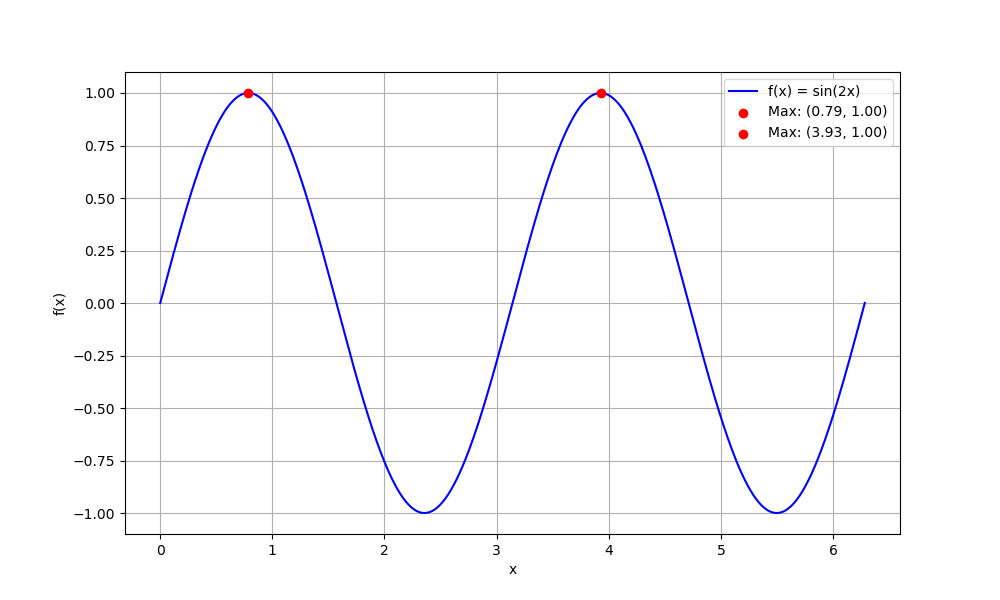
\includegraphics[width=\columnwidth]{figs/gd.png}
    \caption{Plot of \( y = \sin(2x) \) with identified minima and maxima.}
\end{figure}

\end{document}





